\begin{figure}[!ht]
    \centering
    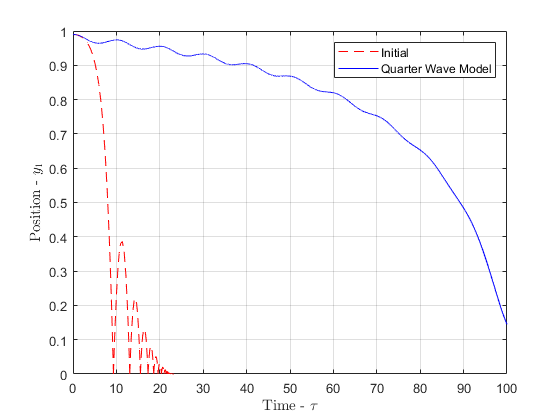
\includegraphics[width=0.4\textwidth]{Figures/QWMSimulation/NearEquilibriumOscillations/Position.png}
    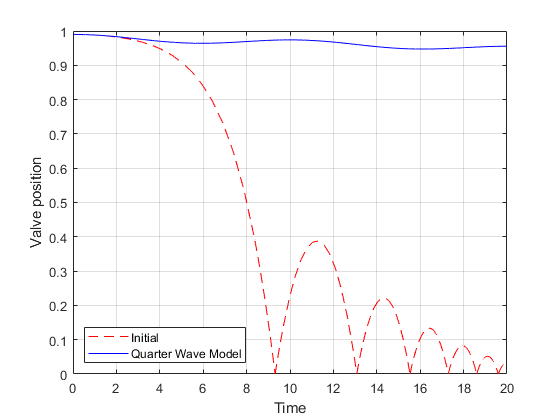
\includegraphics[width=0.4\textwidth]{Figures/QWMSimulation/NearEquilibriumOscillations/Position-Short.png}
    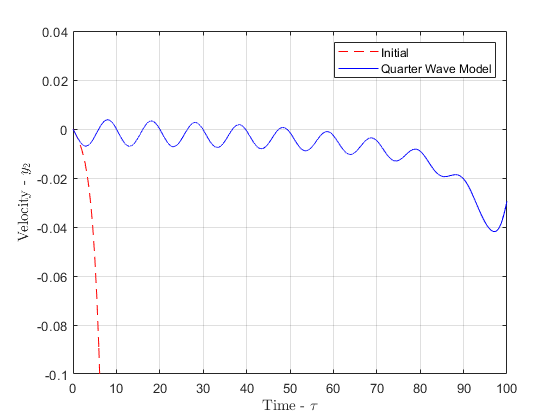
\includegraphics[width=0.4\textwidth]{Figures/QWMSimulation/NearEquilibriumOscillations/Velocity.png}
    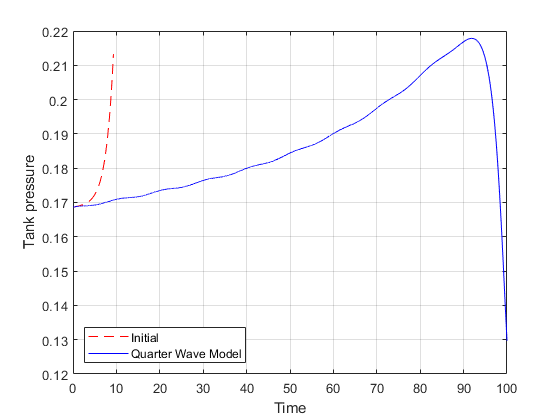
\includegraphics[width=0.4\textwidth]{Figures/QWMSimulation/NearEquilibriumOscillations/Pressure.png}
    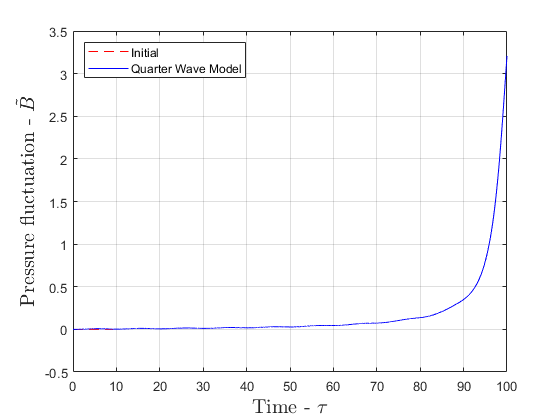
\includegraphics[width=0.4\textwidth]{Figures/QWMSimulation/NearEquilibriumOscillations/B.png}
    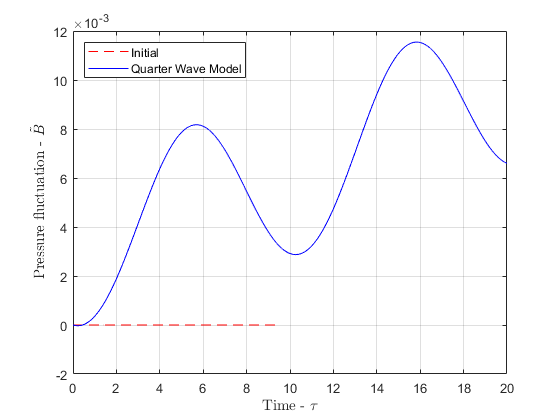
\includegraphics[width=0.4\textwidth]{Figures/QWMSimulation/NearEquilibriumOscillations/B-Short.png}
    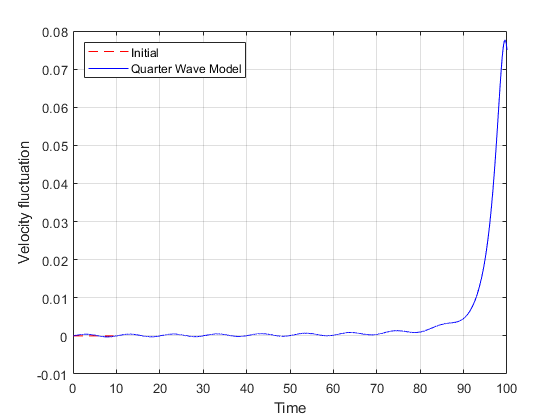
\includegraphics[width=0.4\textwidth]{Figures/QWMSimulation/NearEquilibriumOscillations/C.png}
    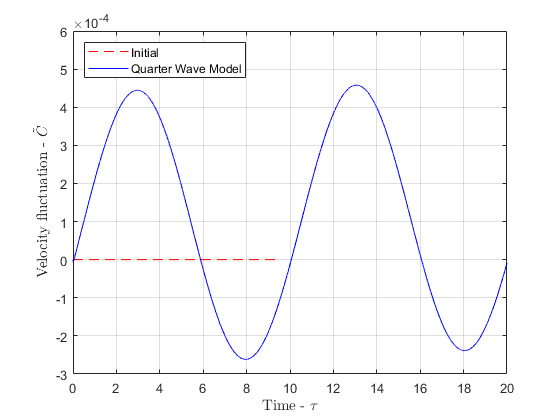
\includegraphics[width=0.4\textwidth]{Figures/QWMSimulation/NearEquilibriumOscillations/C-Short.png}
    % \caption{Simulation of QW with $\gamma = 1.4745$, $q = 0.6$, $\Lambda = 0$, $\alpha = 8.5658$, $\delta = 1$, $\kappa = 0$, $\beta = 0.0433$, $\mu = 0.1407$, $\sigma = 10.3808$, $\phi = 0$ and $r = 0.8$. The initial pressure is the equilibrium pressure of $p = 0.1686$.}
    \caption{Simulation of the full quarter wave model, \cref{eq: FullQWMDimensionless}, for $\gamma = 1.4745$. This can be seen as a blue asterisk [\textcolor{Blue}{$*$}] in \cref{fig: BifurcationDiagram}. The other parameters are as in \cref{tab: ValveClosingQWMParameterValues}, except $\Lambda=0$ and $\phi=0$. The initial conditions are equilibrium values, except $y_1(0) = 0.99$.}
    \label{fig: QWNearEquil}
\end{figure}